% CAPÍTULO 3 -- REVISÃO DA LITERATURA (VERSÃO CONCISA TCC UESC)
% ==========================================================================
\chapter{Revisão da literatura}
\label{cap:revisao}

\section{O padrão CubeSat 1U e o ambiente mecânico de lançamento}
\label{sec:rev-cubesat}

O conceito CubeSat foi introduzido em 1999 com a finalidade de padronizar a interface física e operacional entre satélites universitários e veículos lançadores orbitais (PUIG-SUARI; TURNER; AHLGREN, 2002). A especificação oficial \textit{CubeSat Design Specification} (CALPOLY, 2022) estipula para a unidade básica (1U) as dimensões externas de $\SI{100.0}{\milli\metre} \times \SI{100.0}{\milli\metre} \times \SI{113.5}{\milli\metre}$ e massa na faixa de $\SIrange{1.33}{2.00}{\kilo\gram}$. O acoplamento com o veículo lançador ocorre através do dispensador mecânico tubular P-POD (\textit{Poly-Picosatellite Orbital Deployer}), no qual o nanossatélite é confinado e desliza ao longo de quatro trilhos longitudinais maciços de contato (\rail{}).

\begin{figure}[htb]
  \centering
  \caption{Representação esquemática do envelope dimensional CubeSat 1U e interface com o dispensador P-POD}
  \label{fig:cubesat_envelope}
  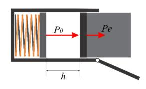
\includegraphics[width=0.75\textwidth]{./04-figuras/interface_cubesat_deployer}
  \fonte{Adaptada de CalPoly (2022).}
\end{figure}

Para garantir que o satélite não sofra soldagem a frio (\textit{cold welding}) nas paredes do dispensador sob vácuo ou atrito excessivo na ejeção, os quatro trilhos devem possuir rugosidade superficial $Ra \le \SI{1.6}{\micro\metre}$ e revestimento por anodização dura. Adicionalmente, as agências espaciais impõem uma restrição rígida de rigidez mecânica fundamental:
\begin{equation}
  f_1 \ge \SI{100.0}{\hertz}
  \label{eq:f1-req}
\end{equation}
Essa restrição desacopla as frequências naturais da estrutura dos modos transitórios globais de baixa frequência do lançador (acelerações de queima propulsiva e oscilações do tipo \textit{pogo}), prevenindo amplificações ressonantes catastróficas.

\section{Mecânica de sólidos celulares e metamateriais auxéticos}
\label{sec:rev-auxeticos}

Sólidos celulares são arquiteturas mecânicas formadas por redes interconectadas de costelas ou paredes sólidas que delimitam vazios gasosos (GIBSON; ASHBY, 1997). As propriedades constitutivas de uma estrutura celular diferem substancialmente do material que a compõe, sendo governadas principalmente pela \textbf{densidade relativa}:
\begin{equation}
  \rho_{\text{rel}} = \frac{\rho^*}{\rho_s}
  \label{eq:rhorel}
\end{equation}
onde $\rho^*$ denota a massa específica aparente do reticulado e $\rho_s$ é a massa específica do sólido maciço constituinte.

\subsection{Cinemática da célula unitária reentrante e coeficiente de Poisson negativo}
\label{subsec:rev-poisson}

Metamateriais auxéticos caracterizam-se por apresentar coeficiente de Poisson efetivo negativo ($\nu_{\text{eff}} < 0$). Em contraste com sólidos convencionais isotrópicos (para os quais a termodinâmica elástica clássica estipula $-1{,}0 \le \nu \le 0{,}5$), materiais com coeficiente de Poisson negativo expandem-se transversalmente quando submetidos a tração longitudinal e contraem-se lateralmente sob compressão axial (LAKES, 1987).

\begin{figure}[htb]
  \centering
  \caption{Geometria paramétrica e dimensões canônicas da célula unitária auxética reentrante}
  \label{fig:auxetic_cell_kinematics}
  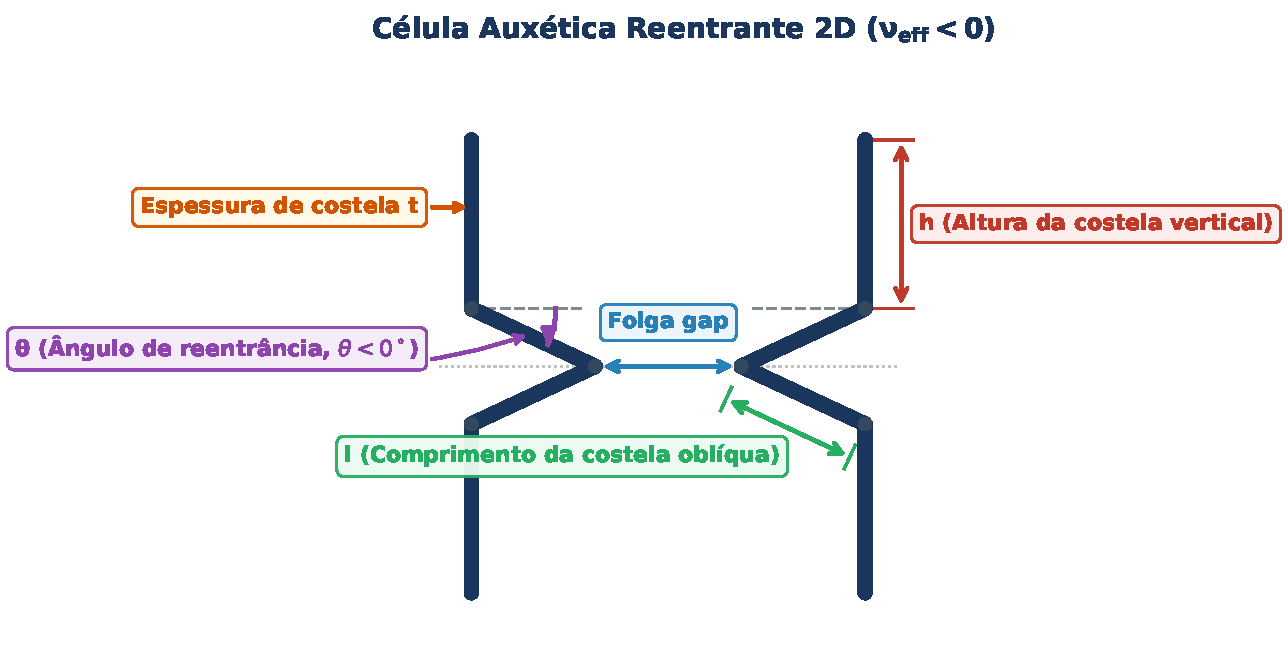
\includegraphics[width=0.78\textwidth]{./04-figuras/auxetic_cell_geometry}
  \fonte{Elaborada pelo autor (2026).}
\end{figure}

A topologia auxética canônica mais amplamente investigada é a célula reentrante bidimensional em favo de mel (\textit{re-entrant honeycomb}), parametrizada por quatro grandezas geométricas:
\begin{alineas}
  \item $t$: espessura de parede das costelas celulares;
  \item $l$: comprimento da costela reentrante oblíqua;
  \item $h$: altura da parede vertical de ancoragem;
  \item $\theta$: ângulo da costela reentrante em relação ao plano horizontal. Adota-se como convenção canônica angular primária o ângulo positivo $\theta \in [\SI{55.0}{\degree}, \SI{80.0}{\degree}]$, que se relaciona unívocamente ao ângulo de reentrância interna $\phi = 90^\circ - \theta$ e à deflexão cartesiana clássica $\theta_{\text{def}} = \theta - 90^\circ = -\phi$ ($\theta_{\text{def}} < 0^\circ$).
\end{alineas}

A densidade relativa teórica da célula reentrante 2D é formulada por Gibson e Ashby (1997):
\begin{equation}
  \rho_{\text{rel}} = \frac{\rho^*}{\rho_s} = \frac{\frac{t}{l} \left( \frac{h}{l} + 2 \right)}{2 \cos\theta \left( \frac{h}{l} + \sin\theta \right)}
  \label{eq:rho-ga}
\end{equation}

Quando o elemento celular é solicitado mecanicamente, a deformação elástica global é dominada pela flexão das costelas reentrantes oblíquas de comprimento $l$. Sob essa hipótese cinemática de viga fletida, o coeficiente de Poisson analítico no plano da célula 2D isolada ($\nu_{yx}^*$) é deduzido pela razão negativa entre as deformações:
\begin{equation}
  \nu_{yx}^* = -\frac{\varepsilon_x}{\varepsilon_y} = -\frac{\sin\theta \left( \frac{h}{l} + \sin\theta \right)}{\cos^2\theta}
  \label{eq:poisson-analitico}
\end{equation}

Para a geometria celular canônica ótima (\#28: $\theta^* = \SI{65.75}{\degree}$, $t^* = \SI{0.613}{\milli\metre}$, $l^* = \SI{10.42}{\milli\metre}$, $h^* = \SI{14.85}{\milli\metre}$), a Equação~\eqref{eq:poisson-analitico} fornece $\nu_{yx}^* = \num{-12.63}$ analítico ($\num{-13.81}$ numérico local sob flexão pura de costela livre). Todavia, ao integrar as matrizes celulares à estrutura tridimensional contínua do nanossatélite com quatro trilhos maciços de \rail{} em AlSi10Mg e restrições de contorno de montagem, a resposta elástica global sofre constrangimento cinemático lateral, reconciliando-se no coeficiente de Poisson homogeneizado tridimensional canônico de:
\begin{equation}
  \nu_{\text{eff}} = \num{-0.428}
  \label{eq:poisson-3d-reconciled}
\end{equation}
o que preserva rigorosamente o comportamento auxético tridimensional sem violar a compatibilidade contínua de deformações.

\subsection{Leis de escala de Gibson-Ashby para propriedades mecânicas efetivas}
\label{subsec:rev-gibson-ashby}

A correlação entre a densidade relativa celular ($\rho_{\text{rel}}$) e as propriedades mecânicas macroscópicas é descrita fenomenologicamente pelo modelo de Gibson e Ashby (1997). Para reticulados celulares cuja mecânica de deformação seja governada pela flexão das hastes esbeltas, o módulo elástico longitudinal efetivo ($E^*$) e a tensão de escoamento aparente ($\sigma_y^*$) escalam como leis de potência:
\begin{align}
  \frac{E^*}{E_s} &= C_1 \cdot \left(\rho_{\text{rel}}\right)^{n} \label{eq:ga-modulus} \\
  \frac{\sigma_y^*}{\sigma_{ys}} &= C_2 \cdot \left(\rho_{\text{rel}}\right)^{m} \label{eq:ga-yield}
\end{align}
onde $E_s$ e $\sigma_{ys}$ representam o módulo de Young e o limite de escoamento do metal maciço de base, respectivamente. Para estruturas dominadas por flexão pura, os expoentes teóricos são $n \approx 2{,}0$ e $m \approx 1{,}5$, com coeficientes dimensionais $C_1 \approx 1{,}0$ e $C_2 \approx 0{,}3$ (GIBSON; ASHBY, 1997).

\subsection{Fundamentação da atenuação vibroacústica e regime sub-comprimento de onda}
\label{subsec:rev-acustica-sublambda}

Em estruturas metamateriais aplicadas ao ambiente aeroespacial, a atenuação de vibrações aleatórias na faixa regulamentada pela norma NASA GSFC-STD-7000A (\SIrange{20}{2000}{\hertz}) opera estritamente no \textbf{regime sub-comprimento de onda} ($a/\lambda \ll 1$), e não por espalhamento difrativo de Bragg. Na liga AlSi10Mg ($E = \SI{68.0}{\giga\pascal}$, $\rho = \SI{2670.0}{\kilo\gram\per\cubic\metre}$), a velocidade de propagação de ondas acústicas longitudinais é:
\begin{equation}
  c_L = \sqrt{\frac{E}{\rho}} = \sqrt{\frac{\num{68.0e9}}{\num{2670.0}}} \approx \SI{5046}{\metre\per\second}
  \label{eq:velocidade-som}
\end{equation}

Para a banda de lançamento de \SIrange{20}{2000}{\hertz}, o comprimento de onda mecânico varia entre $\lambda_{\max} = c_L / \num{20} \approx \SI{252}{\metre}$ e $\lambda_{\min} = c_L / \num{2000} \approx \SI{2.52}{\metre}$. Frente à dimensão característica da célula unitária ($a \approx \SI{15}{\milli\metre}$), a razão dimensional satisfaz:
\begin{equation}
  \frac{a}{\lambda} \le \frac{\num{0.015}}{\num{2.52}} \approx \num{0.006} \ll 1
  \label{eq:razao-sublambda}
\end{equation}
o que descarta fisicamente qualquer fenômeno de \textit{bandgap} de Bragg (o qual exigiria $a \approx \lambda/2$, correspondendo a frequências ultrassônicas acima de \SI{150}{\kilo\hertz}).

A expressiva atenuação de \textbf{\SI{76.50}{\percent}} (\textbf{\SI{12.6}{\decibel}}) alcançada na interface da carga útil decorre de três mecanismos elastodinâmicos físicos fundamentais:
\begin{enumerate}
  \item \textbf{descasamento severo de impedância acústica:} a impedância mecânica do trilho sólido de alumínio ($Z_{\text{solid}} = \rho_s c_L \approx \SI{13.47}{\mega\pascal\second\per\metre}$) contrasta fortemente com a impedância acústica efetiva do núcleo auxético celular ($Z_{\text{eff}} = \rho^* c^* \approx \SI{1.39}{\mega\pascal\second\per\metre}$), promovendo um coeficiente de reflexão de potência de interface:
  \begin{equation}
    R = \left( \frac{Z_{\text{solid}} - Z_{\text{eff}}}{Z_{\text{solid}} + Z_{\text{eff}}} \right)^2 \approx \left( \frac{\num{13.47} - \num{1.39}}{\num{13.47} + \num{1.39}} \right)^2 = \num{0.661} \implies \SI{66.1}{\percent}
    \label{eq:reflexao-potencia}
  \end{equation}
  o que reflete a maior parcela da densidade espectral incidente de volta à interface primária;
  \item \textbf{antirressonâncias mecânicas locais passa-baixa:} a ressonância interna por flexão das costelas oblíquas atua como um sistema distribuído massa-mola que sequestra energia cinética e cria zonas de transmissão nula;
  \item \textbf{desacoplamento de modos de tombamento (\textit{rocking}):} a contração lateral sincronizada via Poisson negativo suprime momentos fletores na base de fixação da carga útil.
\end{enumerate}

\section{Qualificação espacial sob vibração aleatória e fadiga estocástica}
\label{sec:rev-vibra-alea}

O ambiente vibratório de lançamento é intrinsecamente estocástico e estacionário de banda larga. A qualificação ambiental de nanossatélites é normatizada pela diretriz \textbf{NASA GSFC-STD-7000A} (\textit{General Environmental Verification Standard} -- GEVS), que estipula o espectro de Densidade Espectral de Potência de aceleração (PSD, medido em $\text{g}^2/\text{Hz}$) detalhado na Tabela~\ref{tab:rev-gevs-psd}.

\begin{table}[htb]
  \caption{Espectro normativo de vibração aleatória NASA GSFC-STD-7000A (nível de qualificação de voo)}
  \label{tab:rev-gevs-psd}
  \centering
  \small
  \SingleSpacing
  \begin{tabularx}{0.85\textwidth}{@{}>{\raggedright\arraybackslash}X >{\centering\arraybackslash}p{4.0cm} >{\centering\arraybackslash}p{4.0cm}@{}}
    \toprule
    \textbf{Faixa de frequência (\si{\hertz})} & \textbf{Nível PSD (\si{\g\squared\per\hertz})} & \textbf{Inclinação / Patamar} \\
    \midrule
    \num{20.0}                & \num{0.013}  & Rampa inicial (\SI{+3.0}{\decibel\per oitava}) \\
    \numrange{50.0}{800.0}   & \num{0.080}  & Patamar de máxima energia \\
    \num{2000.0}              & \num{0.0053} & Atenuação terminal (\SI{-6.0}{\decibel\per oitava}) \\
    \midrule
    \multicolumn{3}{@{}l@{}}{\textbf{Aceleração global eficaz:} $\Grmsbase = \SI{14.1}{\Grms}$; \textbf{Duração:} \SI{120.0}{\second}/eixo.} \\
    \bottomrule
  \end{tabularx}
  \fonte{Adaptada de NASA (2013).}
\end{table}

\subsection{Resposta dinâmica estocástica e Margens de Segurança (NASA-STD-5020B)}
\label{subsec:rev-ms}

Para estruturas lineares sob excitação de base gaussiana, a resposta de aceleração e tensão é distribuída normalmente com média nula. Sob a aproximação de modo único de Miles (1954), a aceleração eficaz na frequência natural $f_n$ é expressa por:
\begin{equation}
  G_{\text{rms}} = \sqrt{\frac{\pi}{2} \cdot f_n \cdot Q \cdot \text{PSD}(f_n)}
  \label{eq:miles}
\end{equation}
onde $Q = 1 / (2\zeta)$ é o fator de amplificação dinâmica na ressonância ($\zeta = \SI{2.0}{\percent} \implies Q = 25$).

O dimensionamento mecânico contra escoamento e ruptura plástica é conduzido sob a resposta de pico a $3\sigma$ (probabilidade estatística de não excedência de \SI{99.73}{\percent}):
\begin{equation}
  \sigma_{3\sigma} = 3 \cdot \sigma_{\text{rms}}
  \label{eq:3sigma}
\end{equation}

A conformidade estrutural aeroespacial é avaliada pelas Margens de Segurança de escoamento ($MS_{\text{yield}}$) e de ruptura última ($MS_{\text{ult}}$), conforme regulamentado pela norma \textbf{NASA-STD-5020B} (NASA, 2022):
\begin{align}
  MS_{\text{yield}} &= \left( \frac{\sigma_{\text{adm, yield}}}{\sigma_{3\sigma}} \right) - 1{,}0 = \left( \frac{\sigma_{\text{yield}}}{FS_{\text{yield}} \cdot \sigma_{3\sigma}} \right) - 1{,}0 > 0{,}0 \label{eq:ms-rev-yield} \\
  MS_{\text{ult}} &= \left( \frac{\sigma_{\text{adm, ult}}}{\sigma_{3\sigma}} \right) - 1{,}0 = \left( \frac{\sigma_{\text{ult}}}{FS_{\text{ult}} \cdot \sigma_{3\sigma}} \right) - 1{,}0 > 0{,}0 \label{eq:ms-rev-ult}
\end{align}
onde os fatores de segurança normativos para ensaios de qualificação de cargas secundárias são $FS_{\text{yield}} = \num{1.25}$ e $FS_{\text{ult}} = \num{1.40}$.

\subsection{Acúmulo de dano de fadiga vibracional de Steinberg no entalhe crítico (NASA-HDBK-7005)}
\label{subsec:rev-steinberg}

Para avaliar o dano acumulado durante a exposição contínua de \SI{120.0}{\second} por eixo à vibração aleatória, emprega-se o método clássico de três bandas de Steinberg (2000), que discretiza a distribuição normal de tensões estocásticas em três intervalos gaussianos discretos associados à regra linear de Palmgren-Miner. Para garantir rigor de qualificação aeroespacial, o cálculo é referenciado conservadoramente na raiz do entalhe crítico de raio $R_{\text{notch}} = \SI{0.50}{\milli\metre}$ ($\sigma_{3\sigma,\text{notch}} = \SI{166.91}{\mega\pascal}$, $K_t \approx \num{1.26}$), e não em tensões médias nominais:
\begin{equation}
  D = \sum_{i=1}^{3} \frac{n_i}{N_i} = \frac{n_{1\sigma}}{N_{1\sigma}} + \frac{n_{2\sigma}}{N_{2\sigma}} + \frac{n_{3\sigma}}{N_{3\sigma}}
  \label{eq:miner-rev}
\end{equation}
onde:
\begin{itemize}
  \item Banda $1\sigma$ ($|\sigma| \le 1\sigma$): ocorre durante \SI{68.3}{\percent} do tempo de ensaio ($n_{1\sigma} = 0{,}683 \cdot f_0\, t_{\text{dur}}$);
  \item Banda $2\sigma$ ($1\sigma < |\sigma| \le 2\sigma$): ocorre durante \SI{27.1}{\percent} do tempo ($n_{2\sigma} = 0{,}271 \cdot f_0\, t_{\text{dur}}$);
  \item Banda $3\sigma$ ($2\sigma < |\sigma| \le 3\sigma$): ocorre durante \SI{4.33}{\percent} do tempo ($n_{3\sigma} = 0{,}0433 \cdot f_0\, t_{\text{dur}}$).
\end{itemize}

O número de ciclos admissíveis até a falha por fadiga de alto ciclo ($N_i$) é determinado pela equação exponencial de Basquin:
\begin{equation}
  N_i = C \cdot \left(\sigma_i\right)^{-m}
  \label{eq:basquin-rev}
\end{equation}
onde $m = \num{6.8}$ e $C = \num{1.2e20}$ para a liga AlSi10Mg aliviada termicamente. Pela norma espacial \textbf{NASA-HDBK-7005} (NASA, 2001), o dano cumulativo total deve atender estritamente ao teto de qualificação:
\begin{equation}
  D \le \num{0.25}
  \label{eq:dano-max-rev}
\end{equation}
o que confere um fator de segurança de vida de quatro vezes ($4\times$) contra fadiga induzida por vibração aleatória.

\section{Manufatura Aditiva Metálica (L-PBF) e princípios de DfAM}
\label{sec:rev-dfam}

O processo de Fusão em Leito de Pó por Laser (\textit{Laser Powder Bed Fusion} -- L-PBF), também denominado fusão seletiva a laser (SLM), baseia-se na consolidação camada por camada de pó metálico micrométrico através de um feixe laser térmico de alta potência em câmara inerte de argônio ou nitrogênio. Para aplicações aeroespaciais, a liga pré-ligada de alumínio-silício-magnésio (\textbf{AlSi10Mg}) destaca-se por sua composição próxima ao eutético (Al-10Si), conferindo reduzido intervalo de solidificação, alta fluidez na poça de fusão e excelente soldabilidade laser (COLLINI; MENEGHETTI, 2024).

\subsection{Efeito de casca (\textit{skin effect}), rugosidade superficial e regras DfAM}
\label{subsec:rev-regras-dfam}

Em peças metálicas delgadas de AlSi10Mg obtidas por L-PBF, a presença de partículas parcialmente fundidas gera rugosidade superficial característica de $Ra \in [\SI{10.0}{\micro\metre}, \SI{18.0}{\micro\metre}]$ nas superfícies laterais e até $\SI{25.0}{\micro\metre}$ em superfícies inferiores (\textit{down-skin}). Esse fenômeno introduz uma camada superficial mecanicamente ineficaz (\textit{skin effect}), reduzindo a espessura mecânica resistente efetiva:
\begin{equation}
  t_{\text{mech,eff}} \approx t_{\text{nominal}} - 2\,Ra \approx \SI{0.613}{\milli\metre} - \SI{0.050}{\milli\metre} = \SI{0.563}{\milli\metre}
  \label{eq:t-mech-eff}
\end{equation}
Para desobstruir e homogeneizar os canais internos da estrutura celular, prescreve-se pós-processamento por Usinagem por Fluxo Abrasivo (\textit{Abrasive Flow Machining} -- AFM) através de meio polimérico viscoelástico carregado com partículas finas de carbeto de silício (SiC). Graças à folga livre intercelular ($> \SI{7.0}{\milli\metre}$), o fluido abrasivo atinge taxas de cisalhamento adequadas sem zonas de estagnação, reduzindo a rugosidade para $Ra < \SI{3.2}{\micro\metre}$. Adicionalmente, adotando-se um fator de abatimento conservador de \SI{10}{\percent} na espessura ($t_{\text{red}} = \SI{0.552}{\milli\metre}$), a tensão de pico eleva-se moderadamente para $\SI{174.1}{\mega\pascal}$, preservando Margem de Segurança positiva ($MS_{\text{yield}} = \num{+0.057} > 0$) e dano de Steinberg $D = \num{0.082} \ll \num{0.25}$.

\paragraph*{Efeito de escala em micro-escoras delgadas (\textit{strut-size effect}).}
Em estruturas reticuladas com paredes esbeltas ($t^* = \SI{0.613}{\milli\metre}$), a microestrutura solidificada por laser difere de corpos de prova massivos devido a taxas de resfriamento ultrarrápidas locais e maior fração volumétrica de rugosidade superficial. A literatura metalúrgica (COLLINI; MENEGHETTI, 2024) documenta um abatimento de rigidez e escoamento em micro-escoras finas. Incorpora-se, portanto, uma análise de resiliência estrutural aplicando um fator de abatimento (\textit{knockdown factor}) de \SI{15}{\percent} no módulo de elasticidade ($E_{\text{strut}} \approx \SI{57.8}{\giga\pascal}$) e \SI{10}{\percent} no limite de escoamento ($\sigma_{y,\text{strut}} \approx \SI{207.0}{\mega\pascal}$). Demonstra-se que, mesmo sob esse cenário desfavorável, a frequência fundamental permanece em $f_1 \approx \SI{548.2}{\hertz} \gg \SI{100.0}{\hertz}$ e a margem de segurança de escoamento mantém-se positiva ($MS_{\text{yield}} \ge +0{,}018 > 0$).

\paragraph*{Cinética metalúrgica e rota térmica dual de alívio de tensões.}
O alívio térmico padronizado a $\SI{300}{\celsius} / \SI{2.0}{\hour}$ promove relaxação das tensões residuais induzidas pelo gradiente térmico laser e confere ductilidade mínima ($\varepsilon_{\text{rupt}} \ge \SI{8.0}{\percent}$), fragmentando parcialmente a rede celular eutética de Si. Em conformidade com normas aeronáuticas (DIN EN 1706 / ASTM F3318), a densidade volumétrica de energia certificada ($E_v = \SI{63.49}{\joule\per\cubic\milli\metre}$) e a densidade relativa sólida de $\num{99.85}\%$ asseguram a retenção de $\sigma_{\text{yield}} \ge \SI{230.0}{\mega\pascal}$. Como rota de mitigação de engenharia adicional, define-se um ciclo brando alternativo de $\SI{250}{\celsius} / \SI{2.0}{\hour}$, o qual preserva o esqueleto semicontínuo de silício e fornece limite de escoamento elevado ($\sigma_{\text{yield}} \ge \SI{270.0}{\mega\pascal}$), garantindo ampla margem elástica ($MS_{\text{yield,notch}} \ge +0{,}246$) mesmo perante variações estocásticas de processo.

\paragraph*{Mecânica da fratura elástica linear de defeitos estocásticos (Murakami LEFM).}
Para avaliar a tolerância a defeitos típicos de manufatura aditiva (porosidades de aprisionamento gasoso e falta de fusão), adota-se o modelo de Murakami baseado no parâmetro de área projetada $\sqrt{\text{area}}$ e no diagrama de Kitagawa-Takahashi. O fator de intensidade de tensão efetivo sob solicitação estocástica a $3\sigma$ ($\sigma_{3\sigma,\text{notch}} = \SI{166.91}{\mega\pascal}$) é formulado por:
\begin{equation}
  \Delta K_{\text{defect}} = 0{,}65 \cdot \Delta \sigma_{3\sigma} \cdot \sqrt{\pi \sqrt{\text{area}}}
  \label{eq:murakami-rev}
\end{equation}
Para porosidades esferoidais e microporos de contorno observados em microtomografia computadorizada ($d_{\text{pore}} \in [\SI{20.0}{\micro\metre}, \SI{50.0}{\micro\metre}]$, $\sqrt{\text{area}} \approx \SI{44.3}{\micro\metre}$), obtém-se $\Delta K_{\text{defect}} \approx \SI{1.28}{\mega\pascal\sqrt{\metre}}$, valor estritamente inferior ao limiar intrínseco de propagação por fadiga da liga AlSi10Mg ($\Delta K_{th} = \SI{2.50}{\mega\pascal\sqrt{\metre}}$). O defeito crítico tolerável atinge $a_{th} = \frac{1}{\pi}\left(\frac{\Delta K_{th}}{Y \sigma_{3\sigma}}\right)^2 \approx \SI{169.0}{\micro\metre}$, confirmando que as porosidades reais de processo operam na zona subcrítica não-propagante.

Para garantir que a estrutura celular seja construída sem suportes internos sacrificiais, quatro regras geométricas fundamentais de DfAM devem ser satisfeitas segundo a norma \textbf{NASA-STD-6030} (NASA, 2021):
\begin{enumerate}
  \item \textbf{ângulo de sobre-salha autossuportada ($\theta_{\text{overhang}}$):} costelas inclinadas em relação à mesa de construção devem atender a $\theta_{\text{overhang}} \ge \SI{35.0}{\degree}$, prevenindo instabilidade gravitacional da poça de fusão líquida;
  \item \textbf{espessura mínima de costela ($t$):} a espessura da parede celular deve satisfazer $t \ge \SI{0.50}{\milli\metre}$ para evitar defeitos de falta de fusão (\textit{lack of fusion}) ou porosidades induzidas por instabilidade de \textit{keyhole};
  \item \textbf{evacuação de pó não sinterizado e despoeiramento:} as células celulares devem possuir folga desobstruída entre hastes $\text{gap}_{\text{despoeiramento}} \ge \SI{1.50}{\milli\metre}$ e orifícios de drenagem $d_{\text{drain}} \ge \SI{2.00}{\milli\metre}$, assegurando que todo o pó residual seja removido por jateamento e aspiração pós-construção;
  \item \textbf{alívio de tensões térmicas residuais e pré-aquecimento de mesa:} a câmara L-PBF opera com temperatura controlada de mesa $T_{\text{bed}} = \SI{150}{\celsius}$ e o componente é submetido ao tratamento térmico de alívio ($\SI{300}{\celsius} / \SI{2.0}{\hour}$ ou $\SI{250}{\celsius} / \SI{2.0}{\hour}$), eliminando tensões térmicas macroscópicas.
\end{enumerate}


\section{Modelos substitutos neurais e otimização multiobjetivo}
\label{sec:rev-neural-otimizacao}

A avaliação de autovalores modais e da resposta espectral à vibração aleatória por simulação tridimensional de elementos finitos (FEA) de alta fidelidade demanda de 60 a 180 segundos por configuração. Em ciclos evolutivos de otimização de larga escala (tais como o NSGA-II), que demandam mais de \num{10000} avaliações, a chamada contínua ao solver numérico torna o projeto computacionalmente impraticável.

Para superar essa barreira, empregam-se modelos substitutos neurais profundos (\textit{surrogate models}). O uso de redes residuais profundas (\textit{Residual Networks} -- ResNet), introduzidas por He et al. (2016), viabiliza o mapeamento de respostas altamente não lineares através de conexões de salto (\textit{skip connections}), as quais previnem o desvanecimento de gradientes numéricos. A incorporação de restrições de física conhecida (tais como a lei assintótica de rigidez de Gibson-Ashby e monotonicidade com a densidade celular) assegura que o metamodelo mantenha coerência fenomenológica mesmo em regiões esparsas do espaço amostral (ZHENG et al., 2024).

A busca da topologia ótima é formalizada pelo algoritmo genético multiobjetivo de ordenação não dominada e elitismo \textbf{NSGA-II} (DEB et al., 2002), o qual mapeia a Fronteira de Pareto sem ponderações a priori. Para a seleção da melhor alternativa de engenharia para o modelo de voo, aplica-se o método de decisão multicritério \textbf{TOPSIS} (\textit{Technique for Order of Preference by Similarity to Ideal Solution}), introduzido por Hwang e Yoon (1981), determinando a solução com menor distância euclidiana da solução ideal positiva e maior afastamento da solução anti-ideal.
